\documentclass[12pt]{article}
\usepackage[margin=1in]{geometry}
\usepackage{amsmath}
\usepackage{graphicx}

\title{E155 Final Project Status Report: $\mu$Mudd Mark V Debugging and Lab 6 Revision}
\author{Christopher Ferrarin and Kaveh Pezeshki}
\date{28 November 2018}

\begin{document}
	\begin{LARGE}
	\noindent
		E155 
		Final 
		Project 
		Status
		Report: 
		$\mu$Mudd 
		Mark V \\
		Debugging 
		and 
		Lab 
		6 
		Revision
	\end{LARGE}

	\vspace{0.2cm}
	
	\begin{large}
	Christopher Ferrarin and Kaveh Pezeshki
	
	28 November 2018
	\end{large}

\section{Completed Deliverables Status}
To summarize the status of our final project, below is a summary of project deliverables and deliverable status.

	\begin{center}
	\begin{tabular}{p{6cm}p{5cm}p{4cm}}
	Deliverable Category & Deliverable Name & Deliverable Status\\
	\hline
	Identifying blocking $\mu$Mudd Bugs & Identifying MCU programming failure & Complete \\
	Revising $\mu$Mudd to allow MCU functionality & Hardware modification of pre-existing PCBs & Complete \\
	& New JTAG cable & Complete \\
	& Modified schematic and layout & In progress \\
	& Completed and assembled $\mu$Mudd respin & Not started \\
	Reworking Lab 6 & Rewrite EasyPIO.h with SAM4S support & Complete \\
	& Integrate MCP3002, photodiode, and BlueSMiRF & Complete \\
	& Formally write up lab for student readability & Not started \\
	Testing other labs (pending& Lab 4 & Not started \\
	 further discussion)& Lab 5 & Not started \\
	& Lab 7 & Not started
	\end{tabular}
	\end{center}

\section{Deliverable Status: Revised $\mu$Mudd}

A major component of this final project is identifying errors in the PCB design that lead to a non-programmable MCU. We have identified two errors which when solved allowed MCU programming

\subsection{Schematic Errors}

\subsubsection{MCU ERASE Pin}
The largest problem with the current $\mu$Mudd design lies in the MCU ERASE pin, which reinitializes the onboard flash and resets the processor. The ERASE pin can also serve as general-purpose I/O after configuration. \footnote{SAM4S Series Datasheet p37}

On boot, ERASE must be held low to prevent flash erase and reinitialization of the processor. On the current $\mu$Mudd, ERASE was tied to a general I/O pin on the Cyclone IV FPGA. The connection can be seen in the following schematic:

\begin{center}
	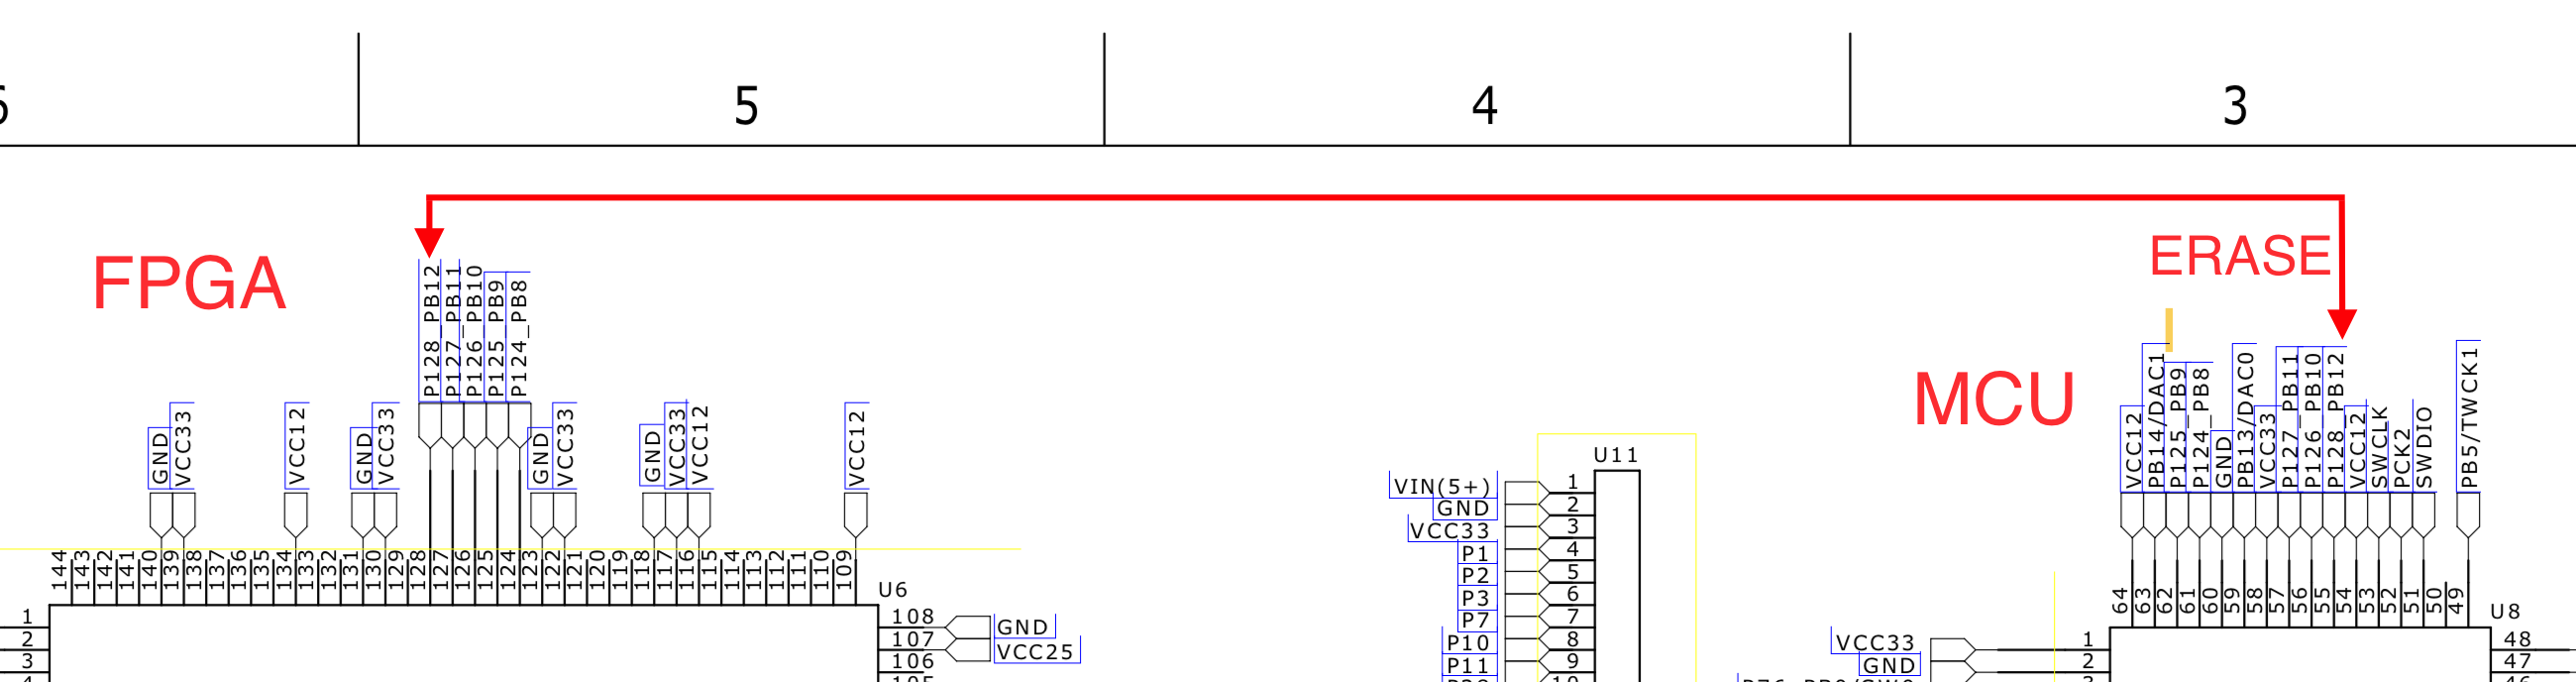
\includegraphics[width=16cm]{erase_error.png}
	\caption{The marked connection ties ERASE on the MCU to pin 128 on the FPGA}
\end{center}

The ERASE pin contains a 100k$\Omega$ pull-down resistor\footnote{SAM4S Series Datasheet p37}.An unconfigured Cyclone IV I/O pin contains a 25k$\Omega$ pull-up resistor \footnote{Cyclone IV Device Handbook p6-3}. This creates a voltage divider circuit as shown below:

\begin{center}
	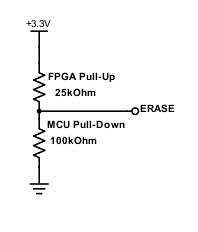
\includegraphics[width=6cm]{resistor_divider.png}
\end{center}

This provides a predicted voltage of 2.64V on the MCU ERASE pin, close to the 2.86V we observed. This is a high logic level which prevented FPGA programming.

\subsubsection{MCU Power Supply}

The MCU requires a 3.3V and 1.2V power supply. It can be powered via one 3.3V supply, and use an internal regulator to generate 1.2V, or it can be powered with an external 3.3V and a 1.2V supply. The dual-regulator design of the current board can introduce startup issues if timing is not correct.

\begin{figure*}
	\begin{center}
	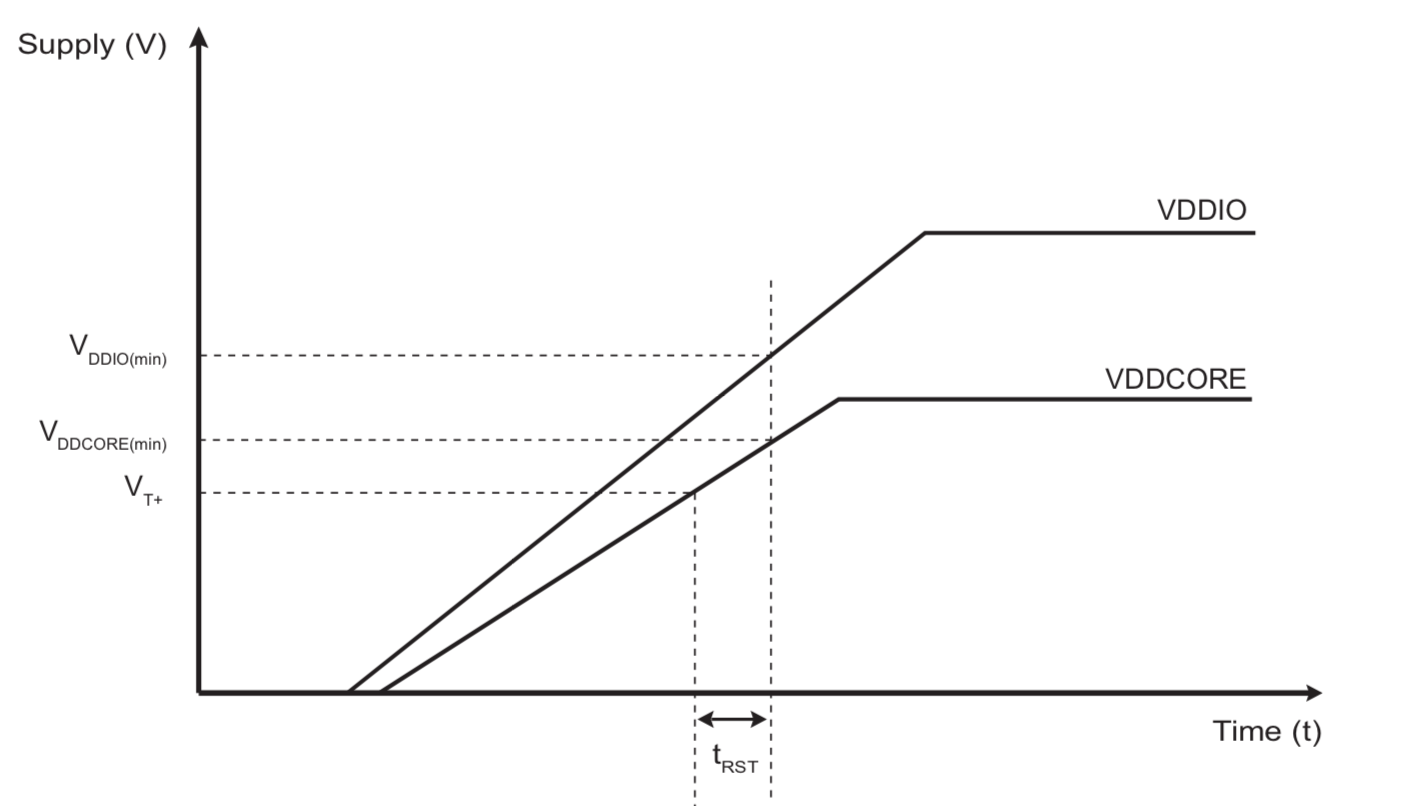
\includegraphics[width=13cm]{power_timing.png}
	\caption{Timing requirements for the 1.2V (VDDCORE) and 3.3V (VDDIO) supplies, taken from the SAM4S Series Datasheet p27}	
	\end{center}
\end{figure*}

We believe that these potential timing errors can cause system instability, as we observed an unresponsive MCU after startup that could only be solved with a full erase and reset.

\subsubsection{JTAG connector pinout}

The MCU JTAG connector was incorrectly wired on the current $\mu$Mudd.

\subsection{Schematic and Layout Changes}

We have implemented a set of changes to the schematic to solve the problems noted above and to improve the PCB, but have not yet propagated these changes to the layout. These include:

\begin{enumerate}
	\item Moving ERASE control to the MCU RESET pushbutton. RESET will be accessible through JTAG
	\item Powering the 1.2V MCU VDDCORE with the onboard regulator
	\item Correcting JTAG wiring errors
	\item Replacing 0.1" pitch JTAG connectors with 0.05" pitch SWD connectors. This adds compatibility with J-Link EDU Mini programmers
\end{enumerate}

\newpage
\section{Deliverable Status: Reworking Lab 6 and EasyPIO.h}

\subsection{Reworking Lab 6}
The proposed Lab 6 architecture is shown in detail below:

\begin{center}
	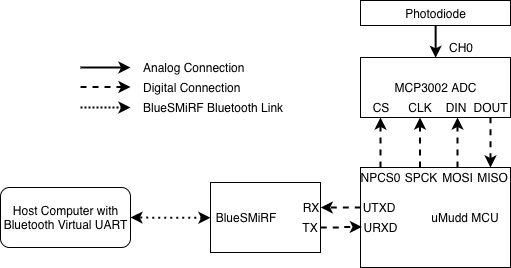
\includegraphics[width=14cm]{blockdiagram.png}
\end{center}

To maintain a low lab cost we exchanged one BlueSMiRF and the serial display for a computer with an integrated Bluetooth module. We added a MCP3002 ADC to retain the datasheet interpretation component of the lab.

We have successfully demonstrated Bluetooth communication between two computers, using a Bus Pirate as a USB to UART converter. We have also successfully demonstrated voltage measurement with the MCP3002 through a SAM3S/SAM4S SPI peripheral.

In reworking Lab 6, we still need to write an updated version of the lab manual and polish it so that it easily readable by a future student. We also seek to implement any recommendations we receive in our presentation for ways to improve this lab, as the replacement of the web server with a Bluetooth link may render the lab simpler than we'd like.

\subsection{Targeting easyPIO.h for the SAM4S}

We have created an I/O header file, easySamIO.h, which provides Arduino-style access to the GPIO, timer, UART, and SPI peripherals on the SAM4S. In the style of easyPIO.h, we provide only the configuration and functionality necessary to complete labs. We aim to provide adequate inline documentation for students to add functionality as necessary. This documentation includes functional descriptions of memory access, references to the lab manual, and brief descriptions of other peripheral features.

In total, we have completed implementation of the PIO, timer, SPI, and UART peripherals, but still need to provide access to additional ports of the PIO peripheral, additional channels of the timer peripheral, and additional clock routing for the FPGA on the $\mu$Mudd.

We believe a thorough and well-documented EasySamIO.h will be more valuable than tests of pre-existing labs as discussed in our project proposal.

\clearpage
\section{Appendix 1: Schematics and Layout}
\clearpage
\section{Appendix 2: C Code}
\subsection{EasySamIO.h}
\begin{tiny}
\begin{verbatim}
// cferrarin@g.hmc.edu
// kpezeshki@g.hmc.edu
// 11/26/2018

// all page numbers reference the SAM4S Series Datasheet as of 11/26/2018

/* This header file simplifies peripheral memory access for the ATSAM4S4B for four peripherals:
1) PMC (Power Management Controller): Controls embeddded system and peripheral clocks. (p418)
In order to use a peripheral, we need to enable its clock in the PMC. p(421)
2) PIO (Parallel I/O Controller): Provides basic GPIO access (turning a pin on or off), or maps GPIO to other peripherals (p467). We implement PIOA here.
3) UART (Universal Asynchronous Receiver/Transmitter): A generic serial controller (p657)
4) SPI (Serial Peripheral Interface): Onboard SPI controller (p582)
5) Timer / Counter: Onboard timer and counter controller (p744)

Before using any of these peripherals, we highly suggest that you read the relevant section in the datasheet. 
We've implemented a bare minimum of configurability and functionality to support the labs, but each peripheral
offers many more features that may prove useful in the final project.
*/



//Constants taken from ATSAM4S4B CMSIS Library
//Relevant code is available at http://packs.download.atmel.com/

/*----------------------------
--------CONSTANTS-------------
----------------------------*/

#define LOW          0
#define HIGH         1

#define INPUT        0
#define OUTPUT       1
#define A            2
#define B            3
#define C            4
#define D            5

#define MCK          4000000
#define TIMER_CLOCK1 (MCK / 2)
#define TIMER_CLOCK4 (MCK / 128)


/*----------------------------
--------REGISTERS-------------
----------------------------*/

//POWER MANAGEMENT CONTROLLER

#define REG_PMC_SCER   (*(  volatile unsigned int *)0x400E0400U) /**< \brief (PMC) System Clock Enable Register */
#define REG_PMC_SCDR   (*(  volatile unsigned int *)0x400E0404U) /**< \brief (PMC) System Clock Disable Register */
#define REG_PMC_SCSR   (*(  volatile unsigned int *)0x400E0408U) /**< \brief (PMC) System Clock Status Register */
#define REG_PMC_PCER0  (*(  volatile unsigned int *)0x400E0410U) /**< \brief (PMC) Peripheral Clock Enable Register 0 */
#define REG_PMC_PCDR0  (*(  volatile unsigned int *)0x400E0414U) /**< \brief (PMC) Peripheral Clock Disable Register 0 */
#define REG_PMC_PCSR0  (*(  volatile unsigned int *)0x400E0418U) /**< \brief (PMC) Peripheral Clock Status Register 0 */
#define REG_CKGR_MOR   (*( volatile unsigned int *)0x400E0420U) /**< \brief (PMC) Main Oscillator Register */
#define REG_CKGR_MCFR  (*(  volatile unsigned int *)0x400E0424U) /**< \brief (PMC) Main Clock Frequency Register */
#define REG_CKGR_PLLAR (*( volatile unsigned int *)0x400E0428U) /**< \brief (PMC) PLLA Register */
#define REG_CKGR_PLLBR (*( volatile unsigned int *)0x400E042CU) /**< \brief (PMC) PLLB Register */
#define REG_PMC_MCKR   (*( volatile unsigned int *)0x400E0430U) /**< \brief (PMC) Master Clock Register */
#define REG_PMC_USB    (*( volatile unsigned int *)0x400E0438U) /**< \brief (PMC) USB Clock Register */
#define REG_PMC_PCK    (*( volatile unsigned int *)0x400E0440U) /**< \brief (PMC) Programmable Clock 0 Register */
#define REG_PMC_IER    (*(  volatile unsigned int *)0x400E0460U) /**< \brief (PMC) Interrupt Enable Register */
#define REG_PMC_IDR    (*(  volatile unsigned int *)0x400E0464U) /**< \brief (PMC) Interrupt Disable Register */
#define REG_PMC_SR     (*(  volatile unsigned int *)0x400E0468U) /**< \brief (PMC) Status Register */
#define REG_PMC_IMR    (*(  volatile unsigned int *)0x400E046CU) /**< \brief (PMC) Interrupt Mask Register */
#define REG_PMC_FSMR   (*( volatile unsigned int *)0x400E0470U) /**< \brief (PMC) Fast Start-up Mode Register */
#define REG_PMC_FSPR   (*( volatile unsigned int *)0x400E0474U) /**< \brief (PMC) Fast Start-up Polarity Register */
#define REG_PMC_FOCR   (*( volatile unsigned int *)0x400E0478U) /**< \brief (PMC) Fault Output Clear Register */
#define REG_PMC_WPMR   (*( volatile unsigned int *)0x400E04E4U) /**< \brief (PMC) Write Protect Mode Register */
#define REG_PMC_WPSR   (*(  volatile unsigned int *)0x400E04E8U) /**< \brief (PMC) Write Protect Status Register */
#define REG_PMC_PCER1  (*(  volatile unsigned int *)0x400E0500U) /**< \brief (PMC) Peripheral Clock Enable Register 1 */
#define REG_PMC_PCDR1  (*(  volatile unsigned int *)0x400E0504U) /**< \brief (PMC) Peripheral Clock Disable Register 1 */
#define REG_PMC_PCSR1  (*(  volatile unsigned int *)0x400E0508U) /**< \brief (PMC) Peripheral Clock Status Register 1 */
#define REG_PMC_OCR    (*( volatile unsigned int *)0x400E0510U) /**< \brief (PMC) Oscillator Calibration Register */

#define PMC_WPMR_WPKEY_PASSWD           (0x504D43u << 8) /**< \brief (PMC_WPMR) Writing any other value in this field aborts 
the write operation of the WPEN bit. Always reads as 0. */


//PARALLEL I/O PORT A

#define REG_PIOA_PER     (*(  volatile unsigned int *)0x400E0E00U) /**< \brief (PIOA) PIO Enable Register */
#define REG_PIOA_PDR     (*(  volatile unsigned int *)0x400E0E04U) /**< \brief (PIOA) PIO Disable Register */
#define REG_PIOA_PSR     (*(  volatile unsigned int *)0x400E0E08U) /**< \brief (PIOA) PIO Status Register */
#define REG_PIOA_OER     (*(  volatile unsigned int *)0x400E0E10U) /**< \brief (PIOA) Output Enable Register */
#define REG_PIOA_ODR     (*(  volatile unsigned int *)0x400E0E14U) /**< \brief (PIOA) Output Disable Register */
#define REG_PIOA_OSR     (*(  volatile unsigned int *)0x400E0E18U) /**< \brief (PIOA) Output Status Register */
#define REG_PIOA_IFER    (*(  volatile unsigned int *)0x400E0E20U) /**< \brief (PIOA) Glitch Input Filter Enable Register */
#define REG_PIOA_IFDR    (*(  volatile unsigned int *)0x400E0E24U) /**< \brief (PIOA) Glitch Input Filter Disable Register */
#define REG_PIOA_IFSR    (*(  volatile unsigned int *)0x400E0E28U) /**< \brief (PIOA) Glitch Input Filter Status Register */
#define REG_PIOA_SODR    (*(  volatile unsigned int *)0x400E0E30U) /**< \brief (PIOA) Set Output Data Register */
#define REG_PIOA_CODR    (*(  volatile unsigned int *)0x400E0E34U) /**< \brief (PIOA) Clear Output Data Register */
#define REG_PIOA_ODSR    (*(  volatile unsigned int *)0x400E0E38U) /**< \brief (PIOA) Output Data Status Register */
#define REG_PIOA_PDSR    (*(  volatile unsigned int *)0x400E0E3CU) /**< \brief (PIOA) Pin Data Status Register */
#define REG_PIOA_IER     (*(  volatile unsigned int *)0x400E0E40U) /**< \brief (PIOA) Interrupt Enable Register */
#define REG_PIOA_IDR     (*(  volatile unsigned int *)0x400E0E44U) /**< \brief (PIOA) Interrupt Disable Register */
#define REG_PIOA_IMR     (*(  volatile unsigned int *)0x400E0E48U) /**< \brief (PIOA) Interrupt Mask Register */
#define REG_PIOA_ISR     (*(  volatile unsigned int *)0x400E0E4CU) /**< \brief (PIOA) Interrupt Status Register */
#define REG_PIOA_MDER    (*(  volatile unsigned int *)0x400E0E50U) /**< \brief (PIOA) Multi-driver Enable Register */
#define REG_PIOA_MDDR    (*(  volatile unsigned int *)0x400E0E54U) /**< \brief (PIOA) Multi-driver Disable Register */
#define REG_PIOA_MDSR    (*(  volatile unsigned int *)0x400E0E58U) /**< \brief (PIOA) Multi-driver Status Register */
#define REG_PIOA_PUDR    (*(  volatile unsigned int *)0x400E0E60U) /**< \brief (PIOA) Pull-up Disable Register */
#define REG_PIOA_PUER    (*(  volatile unsigned int *)0x400E0E64U) /**< \brief (PIOA) Pull-up Enable Register */
#define REG_PIOA_PUSR    (*(  volatile unsigned int *)0x400E0E68U) /**< \brief (PIOA) Pad Pull-up Status Register */
#define REG_PIOA_ABCDSR1 (*(  volatile unsigned int *)0x400E0E70U) /**< \brief (PIOA) Peripheral Select Register */
#define REG_PIOA_ABCDSR2 (*(  volatile unsigned int *)0x400E0E74U) /**< \brief (PIOA) Peripheral Select Register */
#define REG_PIOA_IFSCDR  (*(  volatile unsigned int *)0x400E0E80U) /**< \brief (PIOA) Input Filter Slow Clock Disable Register */
#define REG_PIOA_IFSCER  (*(  volatile unsigned int *)0x400E0E84U) /**< \brief (PIOA) Input Filter Slow Clock Enable Register */
#define REG_PIOA_IFSCSR  (*(  volatile unsigned int *)0x400E0E88U) /**< \brief (PIOA) Input Filter Slow Clock Status Register */
#define REG_PIOA_SCDR    (*(  volatile unsigned int *)0x400E0E8CU) /**< \brief (PIOA) Slow Clock Divider Debouncing Register */
#define REG_PIOA_PPDDR   (*(  volatile unsigned int *)0x400E0E90U) /**< \brief (PIOA) Pad Pull-down Disable Register */
#define REG_PIOA_PPDER   (*(  volatile unsigned int *)0x400E0E94U) /**< \brief (PIOA) Pad Pull-down Enable Register */
#define REG_PIOA_PPDSR   (*(  volatile unsigned int *)0x400E0E98U) /**< \brief (PIOA) Pad Pull-down Status Register */
#define REG_PIOA_OWER    (*(  volatile unsigned int *)0x400E0EA0U) /**< \brief (PIOA) Output Write Enable */
#define REG_PIOA_OWDR    (*(  volatile unsigned int *)0x400E0EA4U) /**< \brief (PIOA) Output Write Disable */
#define REG_PIOA_OWSR    (*(  volatile unsigned int *)0x400E0EA8U) /**< \brief (PIOA) Output Write Status Register */
#define REG_PIOA_AIMER   (*(  volatile unsigned int *)0x400E0EB0U) /**< \brief (PIOA) Additional Interrupt Modes Enable Register */
#define REG_PIOA_AIMDR   (*(  volatile unsigned int *)0x400E0EB4U) /**< \brief (PIOA) Additional Interrupt Modes Disables Register */
#define REG_PIOA_AIMMR   (*(  volatile unsigned int *)0x400E0EB8U) /**< \brief (PIOA) Additional Interrupt Modes Mask Register */
#define REG_PIOA_ESR     (*(  volatile unsigned int *)0x400E0EC0U) /**< \brief (PIOA) Edge Select Register */
#define REG_PIOA_LSR     (*(  volatile unsigned int *)0x400E0EC4U) /**< \brief (PIOA) Level Select Register */
#define REG_PIOA_ELSR    (*(  volatile unsigned int *)0x400E0EC8U) /**< \brief (PIOA) Edge/Level Status Register */
#define REG_PIOA_FELLSR  (*(  volatile unsigned int *)0x400E0ED0U) /**< \brief (PIOA) Falling Edge/Low Level Select Register */
#define REG_PIOA_REHLSR  (*(  volatile unsigned int *)0x400E0ED4U) /**< \brief (PIOA) Rising Edge/ High Level Select Register */
#define REG_PIOA_FRLHSR  (*(  volatile unsigned int *)0x400E0ED8U) /**< \brief (PIOA) Fall/Rise - Low/High Status Register */
#define REG_PIOA_WPMR    (*(  volatile unsigned int *)0x400E0EE4U) /**< \brief (PIOA) Write Protect Mode Register */
#define REG_PIOA_WPSR    (*(  volatile unsigned int *)0x400E0EE8U) /**< \brief (PIOA) Write Protect Status Register */
#define REG_PIOA_SCHMITT (*(  volatile unsigned int *)0x400E0F00U) /**< \brief (PIOA) Schmitt Trigger Register */
#define REG_PIOA_RPR     (*(  volatile unsigned int *)0x400E0F04U) /**< \brief (PIOA) Receive Pointer Register */
#define REG_PIOA_RCR     (*(  volatile unsigned int *)0x400E0F08U) /**< \brief (PIOA) Receive Counter Register */
#define REG_PIOA_RNPR    (*(  volatile unsigned int *)0x400E0F14U) /**< \brief (PIOA) Receive Next Pointer Register */
#define REG_PIOA_RNCR    (*(  volatile unsigned int *)0x400E0F18U) /**< \brief (PIOA) Receive Next Counter Register */
#define REG_PIOA_PTCR    (*(  volatile unsigned int *)0x400E0F24U) /**< \brief (PIOA) Transfer Control Register */
#define REG_PIOA_PTSR    (*(  volatile unsigned int *)0x400E0F28U) /**< \brief (PIOA) Transfer Status Register */

#define PIO_WPMR_WPKEY_PASSWD (0x50494Fu << 8) /**< \brief (PIO_WPMR) Writing any other value in this field aborts the write
operation of the WPEN bit. Always reads as 0. */

//SPI

#define REG_SPI_CR   (*(  volatile unsigned int *)0x40008000U) /**< \brief (SPI) Control Register */
#define REG_SPI_MR   (*(  volatile unsigned int *)0x40008004U) /**< \brief (SPI) Mode Register */
#define REG_SPI_RDR  (*(  volatile unsigned int *)0x40008008U) /**< \brief (SPI) Receive Data Register */
#define REG_SPI_TDR  (*(  volatile unsigned int *)0x4000800CU) /**< \brief (SPI) Transmit Data Register */
#define REG_SPI_SR   (*(  volatile unsigned int *)0x40008010U) /**< \brief (SPI) Status Register */
#define REG_SPI_IER  (*(  volatile unsigned int *)0x40008014U) /**< \brief (SPI) Interrupt Enable Register */
#define REG_SPI_IDR  (*(  volatile unsigned int *)0x40008018U) /**< \brief (SPI) Interrupt Disable Register */
#define REG_SPI_IMR  (*(  volatile unsigned int *)0x4000801CU) /**< \brief (SPI) Interrupt Mask Register */
#define REG_SPI_CSR  (*(  volatile unsigned int *)0x40008030U) /**< \brief (SPI) Chip Select Register */
#define REG_SPI_WPMR (*(  volatile unsigned int *)0x400080E4U) /**< \brief (SPI) Write Protection Control Register */
#define REG_SPI_WPSR (*(  volatile unsigned int *)0x400080E8U) /**< \brief (SPI) Write Protection Status Register */
#define REG_SPI_RPR  (*(  volatile unsigned int *)0x40008100U) /**< \brief (SPI) Receive Pointer Register */
#define REG_SPI_RCR  (*(  volatile unsigned int *)0x40008104U) /**< \brief (SPI) Receive Counter Register */
#define REG_SPI_TPR  (*(  volatile unsigned int *)0x40008108U) /**< \brief (SPI) Transmit Pointer Register */
#define REG_SPI_TCR  (*(  volatile unsigned int *)0x4000810CU) /**< \brief (SPI) Transmit Counter Register */
#define REG_SPI_RNPR (*(  volatile unsigned int *)0x40008110U) /**< \brief (SPI) Receive Next Pointer Register */
#define REG_SPI_RNCR (*(  volatile unsigned int *)0x40008114U) /**< \brief (SPI) Receive Next Counter Register */
#define REG_SPI_TNPR (*(  volatile unsigned int *)0x40008118U) /**< \brief (SPI) Transmit Next Pointer Register */
#define REG_SPI_TNCR (*(  volatile unsigned int *)0x4000811CU) /**< \brief (SPI) Transmit Next Counter Register */
#define REG_SPI_PTCR (*(  volatile unsigned int *)0x40008120U) /**< \brief (SPI) Transfer Control Register */
#define REG_SPI_PTSR (*(  volatile unsigned int *)0x40008124U) /**< \brief (SPI) Transfer Status Register */

#define SPI_WPMR_WPKEY_PASSWD         (0x535049u << 8) /**< \brief (SPI_WPMR) Writing any other value in this field aborts the write
operation of the WPEN bit.Always reads as 0. */

//UART

#define REG_UART_CR   (*(  volatile unsigned int *)0x400E0600U) /**< \brief (UART) Control Register */
#define REG_UART_MR   (*(  volatile unsigned int *)0x400E0604U) /**< \brief (UART) Mode Register */
#define REG_UART_IER  (*(  volatile unsigned int *)0x400E0608U) /**< \brief (UART) Interrupt Enable Register */
#define REG_UART_IDR  (*(  volatile unsigned int *)0x400E060CU) /**< \brief (UART) Interrupt Disable Register */
#define REG_UART_IMR  (*(  volatile unsigned int *)0x400E0610U) /**< \brief (UART) Interrupt Mask Register */
#define REG_UART_SR   (*(  volatile unsigned int *)0x400E0614U) /**< \brief (UART) Status Register */
#define REG_UART_RHR  (*(  volatile unsigned int *)0x400E0618U) /**< \brief (UART) Receive Holding Register */
#define REG_UART_THR  (*(  volatile unsigned int *)0x400E061CU) /**< \brief (UART) Transmit Holding Register */
#define REG_UART_BRGR (*(  volatile unsigned int *)0x400E0620U) /**< \brief (UART) Baud Rate Generator Register */


//TIMER COUNTER 0

#define REG_TC0_CCR  (*(  volatile unsigned int *)0x40010000U) /**< \brief (TC0) Channel Control Register */
#define REG_TC0_CMR  (*(  volatile unsigned int *)0x40010004U) /**< \brief (TC0) Channel Mode Register */
#define REG_TC0_SMMR (*(  volatile unsigned int *)0x40010008U) /**< \brief (TC0) Stepper Motor Mode Register */
#define REG_TC0_CV   (*(  volatile unsigned int *)0x40010010U) /**< \brief (TC0) Counter Value Register */
#define REG_TC0_RA   (*(  volatile unsigned int *)0x40010014U) /**< \brief (TC0) Register A Register */
#define REG_TC0_RB   (*(  volatile unsigned int *)0x40010018U) /**< \brief (TC0) Register B Register */
#define REG_TC0_RC   (*(  volatile unsigned int *)0x4001001CU) /**< \brief (TC0) Register C Register */
#define REG_TC0_SR   (*(  volatile unsigned int *)0x40010020U) /**< \brief (TC0) Status Register */
#define REG_TC0_IER  (*(  volatile unsigned int *)0x40010024U) /**< \brief (TC0) Interrupt Enable Register */
#define REG_TC0_IDR  (*(  volatile unsigned int *)0x40010028U) /**< \brief (TC0) Interrupt Disable Register */
#define REG_TC0_IMR  (*(  volatile unsigned int *)0x4001002CU) /**< \brief (TC0) Interrupt Mask Register */

#define REG_TC_BCR   (*(  volatile unsigned int *)0x400100C0U) /**< \brief (TC) Block Control Register */
#define REG_TC_BMR   (*(  volatile unsigned int *)0x400100C4U) /**< \brief (TC) Block Mode Register */
#define REG_TC_QIER  (*(  volatile unsigned int *)0x400100C8U) /**< \brief (TC) QDEC Interrupt Enable Register */
#define REG_TC_QIDR  (*(  volatile unsigned int *)0x400100CCU) /**< \brief (TC) QDEC Interrupt Disable Register */
#define REG_TC_QIMR  (*(  volatile unsigned int *)0x400100D0U) /**< \brief (TC) QDEC Interrupt Mask Register */
#define REG_TC_QISR  (*(  volatile unsigned int *)0x400100D4U) /**< \brief (TC) QDEC Interrupt Status Register */
#define REG_TC_FMR   (*(  volatile unsigned int *)0x400100D8U) /**< \brief (TC) Fault Mode Register */
#define REG_TC_WPMR  (*(  volatile unsigned int *)0x400100E4U) /**< \brief (TC) Write Protect Mode Register */

#define TC_WPMR_WPKEY_PASSWD (0x54494Du << 8) /**< \brief (TC_WPMR) Writing any other value in this field aborts the write
operation of the WPEN bit. Always reads as 0. */

void samInit() {
//Many peripherals on the SAM4S are write protected: unless the correct password is written in a peripheral memory address, 
write access to peripheral control registers is disabled. This is done for security reasons, but is not necessary in this header file.
In the first part of this function, we enable write access to the PMC, PIO, SPI, and UART by writing a password into the peripheral's 
Write Protect Mode Register (WPMR)


//disabling PMC write protection (Password: "PMC")
REG_PMC_WPMR = PMC_WPMR_WPKEY_PASSWD;
//disabling PIO write protection (Password: "PIO")
REG_PIOA_WPMR = PIO_WPMR_WPKEY_PASSWD;
//disabling SPI write protection (Password: "SPI")
REG_SPI_WPMR = SPI_WPMR_WPKEY_PASSWD;
//There is no UART write protection

//disabling timer write protection (Password: "TIM")
REG_TC_WPMR = TC_WPMR_WPKEY_PASSWD;

//We next need to supply a clock to these peripherals. For a given peripheral, clock is enabled by writing a 1 into a specific bit
of the PMC Peripheral Clock Enable Register (PCER). There are two registers for the 34 peripherals. Peripheral - bit number mapping
is given in p36: Peripheral Identifiers.

//Activating clocks for UART 0 (PID 8), PIO A (PID 11), SPI (PID 21), TC0 (Timer/Counter CH0) (PID 23)

REG_PMC_PCER0 |= (1<<8);
REG_PMC_PCER0 |= (1<<11);
REG_PMC_PCER0 |= (1<<21);
REG_PMC_PCER0 |= (1<<23);
}


/*----------------------------
--------PIO METHODS-------------
----------------------------*/

void pinMode(int pin, int function) {
REG_PIOA_IFDR  |=  (1 << pin);
REG_PIOA_IER   &= ~(1 << pin);
REG_PIOA_IDR   |=  (1 << pin);
REG_PIOA_MDER  &= ~(1 << pin);
REG_PIOA_MDDR  |=  (1 << pin);
REG_PIOA_PUER  &= ~(1 << pin);
REG_PIOA_PUDR  |=  (1 << pin);
REG_PIOA_PPDER &= ~(1 << pin);
REG_PIOA_PPDDR |=  (1 << pin);
REG_PIOA_OWER  &= ~(1 << pin);
REG_PIOA_OWDR  |=  (1 << pin);

if (function == INPUT || function == OUTPUT) {
REG_PIOA_PER |=  (1 << pin);
REG_PIOA_PDR &= ~(1 << pin);
} else {
REG_PIOA_PER &= ~(1 << pin);
REG_PIOA_PDR |=  (1 << pin);
}

switch (function) {
case INPUT:
REG_PIOA_OER &= ~(1 << pin);
REG_PIOA_ODR |=  (1 << pin);
break;
case OUTPUT:
REG_PIOA_OER |=  (1 << pin);
REG_PIOA_ODR &= ~(1 << pin);
break;
case A:	
REG_PIOA_ABCDSR1 &= ~(1 << pin);
REG_PIOA_ABCDSR2 &= ~(1 << pin);
break;
case B:
REG_PIOA_ABCDSR1 |=  (1 << pin);
REG_PIOA_ABCDSR2 &= ~(1 << pin);
break;
case C:
REG_PIOA_ABCDSR1 &= ~(1 << pin);
REG_PIOA_ABCDSR2 |=  (1 << pin);
break;
case D:
REG_PIOA_ABCDSR1 |= (1 << pin);
REG_PIOA_ABCDSR2 |= (1 << pin);
break;
// Otherwise, do nothing
}
}

void digitalWrite(int pin, int val) {
if (val == HIGH) {
REG_PIOA_SODR |= (1 << pin);
} else {
REG_PIOA_CODR |= (1 << pin);
}
}

int digitalRead(int pin) {
return (REG_PIOA_PDSR >> pin) & 1;
}

void toggle(int pin) {
int currentVal = digitalRead(pin);
digitalWrite(pin, !currentVal);
}


/*----------------------------
--------SPI METHODS-------------
----------------------------*/

void spiInit(char clkdivide, int cpol, int ncpha) {
/*Initializes the SPI interface for Chip Select line 0

clkdivide (0x01 to 0xFF). The SPI clk will be the master clock / clkdivide
cpol: clock polarity (0: inactive state is logic level 0, 1: inactive state is logic level 1)
ncpha: clock phase (0: data changed on leading edge of clk and captured on next edge, 1: data captured on leading edge of clk and changed on next edge)
Please see p585-p586 for cpol/ncpha timing diagrams

This implements only: (p601/p610)
1) SPI Master Mode
2) Fixed Peripheral Select
3) Mode Fault Detection Enabled
4) Local Loopback Disabled
5) 8 Bits Per Transfer
Please read the SPI User Interface section of the datasheet for more advanced configuration features
*/

//Initially assigning SPI pins (PA11-PA14) to peripheral A (SPI). Pin mapping given in p38-p39
pinMode(11, A);
pinMode(12, A);
pinMode(13, A);
pinMode(14, A);

//next setting the SPI control register (p600). Set to 1 to enable SPI
REG_SPI_CR = 1;

//next setting the SPI mode register (p601) with the following:
//master mode
//fixed peripheral select
//chip select lines directly connected to peripheral device
//mode fault detection enabled
//WDRBT disabled
//LLB disabled
//PCS = 0000 (Peripheral 0 selected), means NPCS[3:0] = 1110
REG_SPI_MR = 1;

//next setting the chip select register for peripheral 0 (p610)
//ignoring delays

//REG_SPI_CSR = (cpol<<0) | (ncpha<<1) | (clkdivide << 16);
REG_SPI_CSR = 0x0000FF00;
}

char spiSendReceive(char send) {
//Sends one byte over SPI and returns the received character
REG_SPI_TDR = send;
//Wait until Receive Data Register Full (RDRF, bit 0) and TXEMPTY (bit )
while ( !( (REG_SPI_SR & 1) & ((REG_SPI_SR >> 9) & 1) ) );
//After these status bits have gone high, the transaction is complete  
return REG_SPI_RDR;
}

short spiSendReceive16(short send) {
//sends one 16-bit short over SPI and returns the received short
short rec;
rec = spiSendReceive((send & 0xFF00) >> 8); // send data MSB first
rec = (rec << 8) | spiSendReceive(send & 0xFF);
return rec;
}


/*----------------------------
--------TIMER METHODS-------------
----------------------------*/

void timerInit() {
// Enable clock to channel
REG_TC0_CCR	   &= ~(1 << 1);
REG_TC0_CCR	   |= 1;

REG_TC0_CMR    |= (1 << 15); // WAVE = 1 (waveform mode)
REG_TC0_CMR	   |= (1 << 14); // WAVESEL = 2 (UP_RC waveform)
}

// Works until 2097 ms
// Resolution of 32 us
void delay_ms(int num) {
REG_TC0_CMR |= 0x3; //0b11; // Using TIMER_CLOCK4
REG_TC0_RC   = (unsigned long) (TIMER_CLOCK4 * (((float) num) / 1000)); // Compare value
REG_TC0_CCR |= (1 << 2); // Reset counter
while (!((REG_TC0_SR >> 4) & 1)); // Delay until match
}


/*----------------------------
--------UART METHODS-------------
----------------------------*/

/* Initialize UART. Note that pin PA9 is used as receive and pin PA10 
* is used as transmit. samInit() must be called first.
* parity:
*	 0: Even
*	 1: Odd
*	 2: Space (forced to 0)
*	 3: Mark (forced to 1)
*	 4: No (no parity)
* Baud Rate =  MCK/(16*CD), CD is an unsigned short
*/	
void uartInit(int parity, int CD) {
pinMode(9, A);		  // Set URXD0 pin mode
pinMode(10, A);		  // Set ITXD0 pin mode

REG_UART_CR   |= 1 << 6; // Enable transmitter
REG_UART_CR   |= 1 << 4; // Enable receiver

// Parity
//REG_UART_MR   |= parity << 9;    
//REG_UART_MR   &= ~(parity << 9);
REG_UART_MR   |= 1 << 11;
REG_UART_MR   &= ~((0x3) << 9);

REG_UART_BRGR = CD;	  // Set baud rate divider
}

// Transmits a character (1 byte) over UART
void uartTx(char data) {
while (!((REG_UART_SR >> 1) & 1)); // Wait until previous data has been transmitted
REG_UART_THR = data; // Write data into holding register for transmit
}

// Returns a character (1 byte) received over UART
char uartRx() {
while(!((REG_UART_SR) & 1)); // Wait until data has been received
return (char) REG_UART_RHR; // Return received data in holding register

}

\end{verbatim}
\end{tiny}

\pagebreak
\subsection{lab6.c}
\begin{scriptsize}
\begin{verbatim}
#include <easySamIO.h>
#include <stdio.h>

int main() {
samInit();
uartInit(4, 2);
timerInit();
spiInit(255, 0, 0);
pinMode(17, OUTPUT);

unsigned short received = 0;
float voltage;
char strTransmit[5];
char introTransmit[10] = "Voltage: ";

while (1) {
digitalWrite(17, HIGH);

received = spiSendReceive16(0x6000);
received &= 0x03FF; // Removing 6 MSbs
voltage = 3.3 * ((float) received / 1023.0);

snprintf(strTransmit, 5, "%f", voltage);

for (int charNum = 0; charNum < 9; charNum++) {
uartTx(introTransmit[charNum]);
}

for (int charNum = 0; charNum < 5; charNum++) {
uartTx(strTransmit[charNum]);
}

uartTx(0x0A);

digitalWrite(17, LOW);

delay_ms(1000);
}
return 1;
}
\end{verbatim}
\end{scriptsize}
	
\end{document}
